\phantomsection
\chapter{Feature Extraction with Local Binary Patterns}
\label{chap:implementation_lbp}

\noindent As said previously, the Local Binary Patterns (LBP) method is used as feature extraction method for this Facial Expression Recognition system. This chapter describes how this method is used and implemented.
\newline

\phantomsection
\section{Uniform Local Binary Patterns}

\vspace{\baselineskip}
\noindent A circular uniform LBP operator, $ LBP_{8,1}(p) $, is used with a number of neighbours $ P = 8 $ and radius $ R = 1.0 $ to compute pixel values of the image. The figure~\ref{lbp_implementation_example} shows what is obtained with this operator. 
\newline

\begin{figure}[!h]
\begin{center}
\noindent 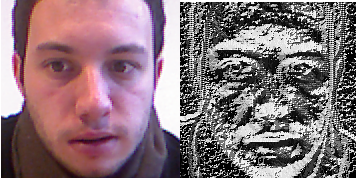
\includegraphics[scale=0.8]{figures/lbp_implementation_example} 
\newline
\caption{Circular LBP operator with $ P = 8 $ and $ R = 1.0 $}
\label{lbp_implementation_example}
\end{center} 
\end{figure}

\noindent The face image is divided into regions. As it is commonly done, the face is a grid pattern of $ 7\times6 $ (7 partitions for the rows and 6 partitions for the columns). In total the face image is divided into 42 regions. For each of these regions, the LBP operator, $ LBP_{8,1}^{u^2} $, computes every pixel.
\newline

\noindent The output of this computation is the number of labelled 1s in the 8-pixels neighourhood. Because a uniform LBP operator is used, values range from 0 to 8. There can also be an output of 9, if this is a non-uniform LBP pattern. To sum up, the output number can have 10 different values (from 0 to 9).
\newline

\phantomsection
\section{Histogram computing}

\vspace{\baselineskip}
After obtaining all pixel values from a region, they are concatenated into a 10-bin histogram, one for each value from 0 to 9. Each bin contains the number of pixels having the value corresponding to that bin. For example, if in a specific region, 20 pixels are labelled with the value 7 after being computed by the LBP operator, then the bin attributed to the value 7 will have a value of 20 for this specific region. Figure~\ref{lbp_implementation_histogram} shows two pixels with their eight neighbor pixels, a region containing these pixels with the values obtained with the LBP operator and an histogram computed for this region.
\newline

\begin{figure}[!h]
\begin{center}
\noindent 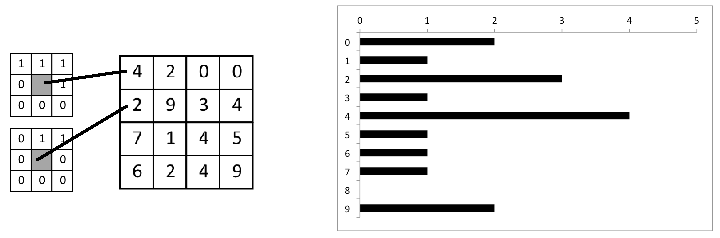
\includegraphics[scale=0.6]{figures/lbp_implementation_histogram} 
\newline
\caption{Example of Histogram computation}
\label{lbp_implementation_histogram}
\end{center} 
\end{figure}

\noindent To obtain the feature vector for the whole image, an histogram is computed for each region. Thus, 42 histograms are computed for the 42 regions. Since eeach histogram has 10 bins, the concatenation of all histograms outputs a feature vector of 420 points. Figure~\ref{lbp_implementation_vector} shows how the feature vector is obtained with all the histograms.
\newline

\begin{figure}[!h]
\begin{center}
\noindent 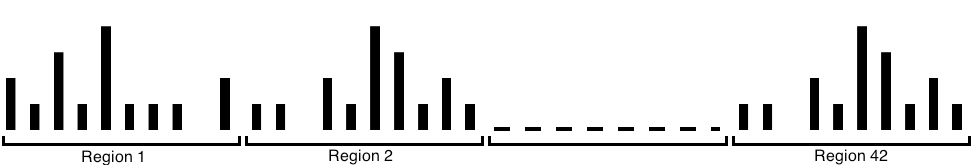
\includegraphics[scale=0.4]{figures/lbp_implementation_vector} 
\newline
\caption{Example of a feature vector composed by the 42 histograms}
\label{lbp_implementation_vector}
\end{center} 
\end{figure}

